\chapter{Evaluation}\label{ch:evaluation}
\section*{Vergleich genetischer Operatoren}
Zunächst wollen wir uns einen Überblick über die verschiedenen genetischen Operatoren verschaffen und diese vergleichen. Zu diesem Zweck wurden 1000 hidden Markov Modelle zufällig erstellt welche dann 20 Iterationen des Baum-Welch Algorithmus angewendet wurde. Der Observationssequenzen stammen hierbei aus dem Free Spoken Digit Dataset. Nach jedem Schritt des BW-Algorithmus wurden die verschiedenen Crossover und Mutationsoperatoren angewendet. So wurde die durchschnittliche Wahrscheinlichkeit ermittelt, dass ein gegebener Mutationsoperator ein Chromosom mit höherer Fitness erzeugt. Für die Crossoverfunktion wurde die durchschnittliche Wahrscheinlichkeit ermittelt, dass ein Kind eine höhere Fitness als seine Eltern hat.

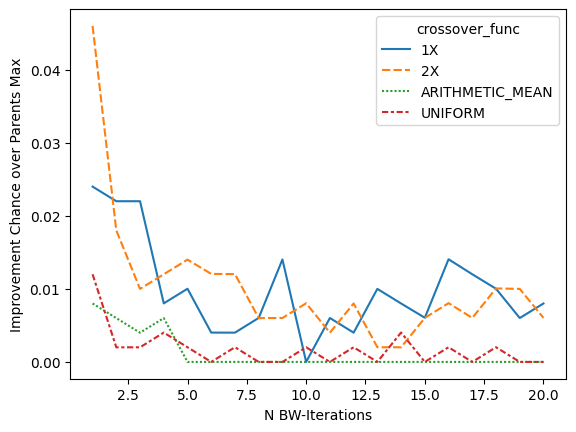
\includegraphics[width=0.5\linewidth]{images/charts/crossover_function_improvement_chance_parents_max.png}
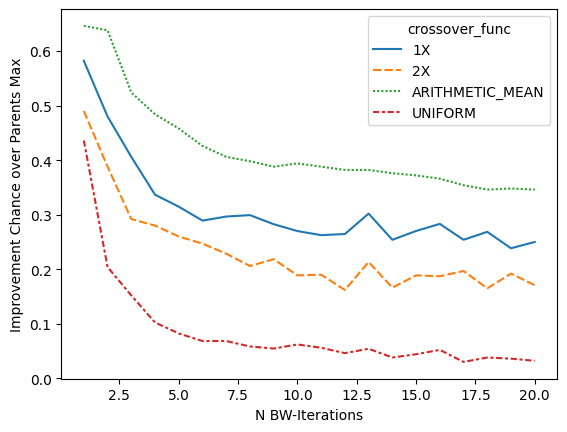
\includegraphics[width=0.5\linewidth]{images/charts/crossover_function_improvement_chance_parents_min.png}

Wir können beobachten: je fitter die Eltern sind, desto geringer ist die Wahrscheinlichkeit, dass das Kind eine höhere Fitness als seine Eltern hat. Der Arithmetic Mean Crossover hat die höchste Wahrscheinlichkeit ein Kind zu erzeugen, welches eine höhere Fitness als ein mindestens ein Elternteil hat. Interessanterweise scheint der Arithmetic Mean Crossover jedoch nicht in der Lage zu sein Kinder zu Erzeugen, welche eine höhere Fitness als \textit{beide} Elternteile haben. Der Uniforme Crossover schneidet am schlechtesten von allen ab und sollte nicht als Crossoveroperator eingesetzt werden. Der Single Point Crossover schlägt sich insgesamt am besten und wird im folgenden weiter betrachtet. 

Eine Auswertung mit den selben Parametern wurde auch für die Mutationsoperatoren unternommen. Vergleicht wurde eine uniforme Mutation mit verschiedenen Werten für die Mutationschance. Es wurden die Werte 0.1, 0.01 und 0.001 als Mutationschance verglichen. Figur [MOPED] zeigt, Wahrscheinlichkeit, dass die Fitness eines Chromosoms nach der Mutation höher ist als zuvor abhängig von dem Grad der Optimierung (Anzahl der BW-Iterationen). Nur eine Mutationsrate von 0.001 ist verlässlig in der Lage Chromosome zu erzeugen, welche nach der Mutation eine höhere Fitness aufweisen. Figur [MOPED2] zeigt die durchschnittliche Fitness nach der Mutation im Vergleich zu keiner Mutation (nur Baum-Welch). Erneut beobachten wir, dass eine geringe Mutationsrate wünschenswert ist, da die Fitness der Population sonst enorm sinkt.
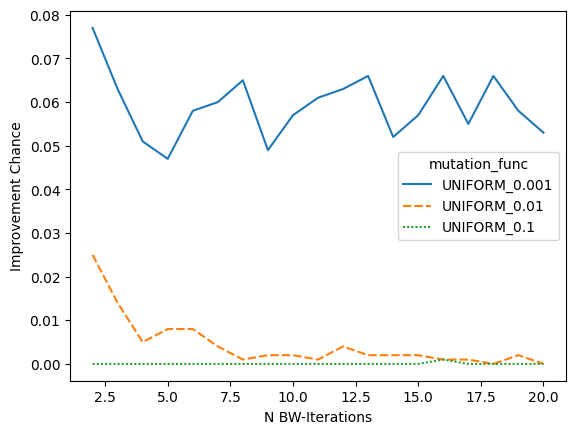
\includegraphics[width=0.5\linewidth]{images/charts/mutation_function_improvement_chance.png}
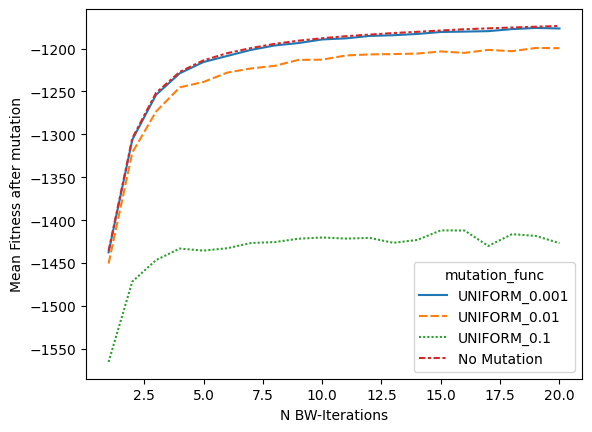
\includegraphics[width=0.5\linewidth]{images/charts/mean_fitness_after_mutation.png}

Natürlich ist solch ein isolierter Vergleich nur bedingt Aussagekräftig, da hier mögliche Interaktionseffekte der genetischen Operatoren nicht beachtet werden. Die Auswertung gibt uns jedoch eine Intuition über die Effektivität der Crossover- und Mutationsoperatoren. Bereits ab 5 BW-Iterationen, also schon ab einem geringen Maß an Optimierung, sinkt die Wahrscheinlichkeit ein Kind zu erzeugen, welches fitter als beide Eltern ist auf unter 2\% für den single Point Crossover. Gleichzeitig liegt die Wahrscheinlichkeit mittels single Point Crossover ein Kind zu erzeugen, welches schlechter als beide Eltern ist nach 5 BW-Iterationen bei über 96\%. Wir sehen also, dass der größte Teil unserer Rechenzeit dafür verwendet wird weniger optimierte Lösungen zu erzeugen.

\section*{Eine Käsestudie (Case Study)}
In diesem Abschnitt werden wir das GA-HMM Framework verwenden um einen existierenden Ansatz für die hybride Parameter-Estimation zu evaluieren. Der Ansatz welchen wir betrachten ist ,,Optimizing Hidden Markov Models with a Genetic Algorithm" ~\cite*{LiteratureEvalGASlimane} von M. Slimane et al aus dem Jahr 1996. Dieses Paper wurde unter anderem ausgewählt, da es sich um einen der ältesten und meist zitierten Ansätze unter den hybriden Verfahren zur HMM-Parameter-Estimation handelt. Die Autoren verwenden einen genetischen Algorithmus um initiale Parameter für den Baum-Welch Algorithmus zu ermitteln. Es handelt sich also um einen Relay-Hybriden Ansatz. Es wurden 10 Observationssequenzen mit Längen zwischen 8 und 12 Observationen verwendet. Die Anzahl der Observationssymbole variiert zwischen 2 und 6.
Als Strategie werden folgende Parameter verwendet
\begin{itemize}
    \item Populationsgröße 60
    \item Elitismus 30
    \item Anzahl GA-Iterationen 200
    \item Selektionsstrategie Uniform zufällig
    \item Selektionsmenge: Die besten 30 Individuen
    \item Crossoveroperator: Single Point Crossover, jedoch nur am Ende von Reihen (1X)
    \item Mutationsoperator: Uniform Random Mutation
    \item Mutationschance: 0.01
    \item Rekombinationsstrategie: Generation wird bis auf Eliten komplett ersetzt
    \item Anzahl BW-Iterationen: 50
\end{itemize}
Parameterinitialisierungsstrategie besteht darin den ersten Parameter jeder Reihe beliebig im Interval $[0,1]$ zu wählen und die folgenden parameter aus dem Intervall $[0,x]$, wobei $x$ die Summe der vorherigen Parameter in der Reihe ist.

In ihren Auswertung bereichten Slimane et al, dass der hybride Ansatz im Durchschnitt bessere Hidden Markov Modelle erstellt. 
Ich konnte diese Ergebnisse verifizieren

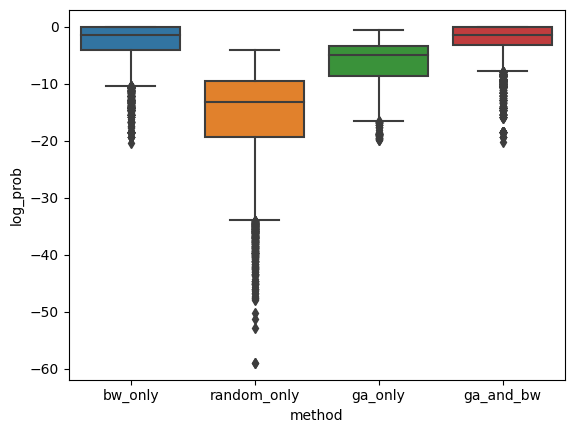
\includegraphics[width=0.5\linewidth]{images/charts/slimane_log_prob_comparison.png}
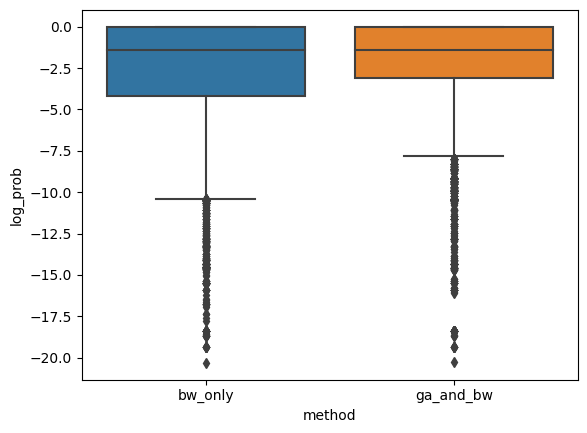
\includegraphics[width=0.5\linewidth]{images/charts/slimane_log_prob_comparison_showdown.png}

Wir sehen, dass der genetische Algorithmus tatsächlich in der Lage ist im Durchschnitt bessere Ergebnisse zu finden als eine einfache Anwendung des BW-Algorithmus. Ein großer Nachteil des genetischen Algorithmus ist jedoch, dass er sehr Rechenintensiv ist. Grafik [SCHMOPED1] zeigt einen vergleich der durchschnittlichen Berechnungszeiten für eine Anwendung der jeweiligen Strategien. Die Durchführung des hybriden Algorithmus dauert durchschnittlich 0.997 Sekunden. Eine Anwendung von BW-Algorithmus alleine dauert durchschnittlich lediglich 0.002 Sekunden. Der hybride Algorithmus ist somit über 480x langsamer als der Baum-Welch Algorithmus alleine.
Zu diesen Werten muss allerdings angeführt werden, dass der Baum-Welch Algorithmus vollständig optimiert ist und der genetische Teil des GA-HMM nur Teilweise optimiert. Andererseits ist ein genetischer Algorithmus einfach schwieriger zu optimieren, da man im Vergleich zum BW-Algorithmus enorm viele Parameter und Optionen verwalten muss. Ich bezweifle daher, dass eine weitaus performantere Implementation des genetischen Algorithmus möglich ist ohne dabei die Flexibilität und Lesbarkeit des Codes zu komprimieren. Dass der hybride genetische Algorithmus viel mehr Zeit benötigt ist per se kein Ausschluss-Kriterium. Auch wenn der hybride Algorithmus viel mehr Zeit benötigt, so ist eine maximale Rechendauer von unter 5 Sekunden wohl tollerierbar. Was uns interessieren sollte ist ob der hybride Algorithmus in der Lage ist Lösungen zu finden, welche ein reiner BW-Algorithmus in der selben Rechenzeit nicht finden kann. Um das zu überprüfen habe ich eine Anwendung des hybriden Algorithmus verglichen mit dem maximalen Wert aus N unabhängigen BW Anwendungen, wobei N von 1 bis 30 geht. Figur [SCHMOPED2] zeigt die Mittelwerte der Maximalen Fitness aus N BW Anwendungen. Der Mittelwert des hybriden Ansatzes ist ebenfalls als Referenz eingezeichnet. Wir sehen, dass bereits drei Anwendungen des BW-Algorithmus ausreichen um im Durchschnitt bessere Ergebnisse als der hybride Ansatz zu erzielen. Durch eine Erhöhung der Anzahl an BW Anwendungen kann die durchschnittliche Wahrscheinlichkeit sogar noch weiter erhöht werden. Durch mehrfache Anwendung des BW Algorithmus und wählen des wahrscheinlichsten Modells können wir also bessere Ergebnisse als durch den hybriden Ansatz für einen Bruchteil der Rechenzeit erhalten.

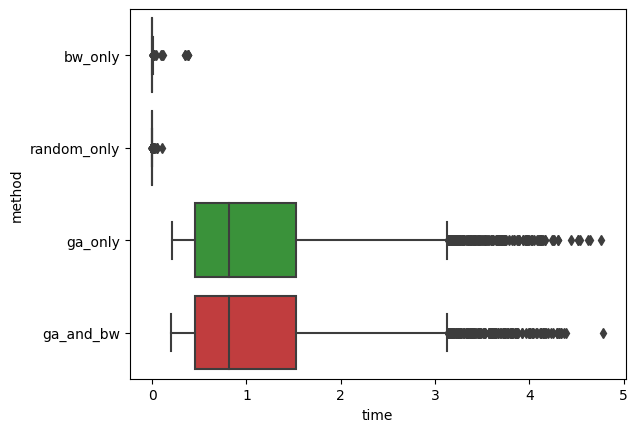
\includegraphics[width=0.5\linewidth]{images/charts/slimane_execution_time.png}
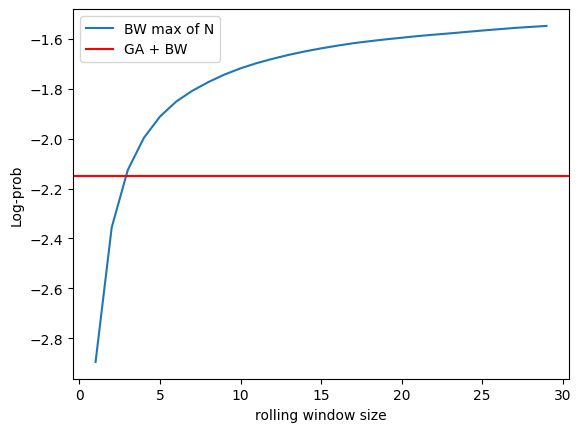
\includegraphics[width=0.5\linewidth]{images/charts/slimane_rolling_window.png}


% \begin{figure}
%     \begin{sub
% \end{figure}
% \begin{figure}
%     % \begin{subfigure}
%     %     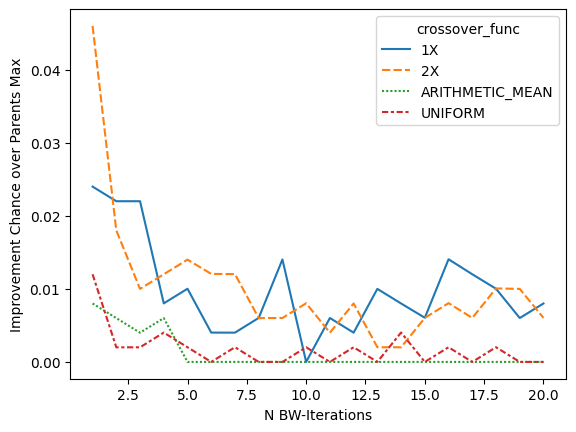
\includegraphics[scale=1.0]{images/charts/crossover_function_improvement_chance_parents_max.png}
%     %     \caption{soooos}
%     % \end{subfigure}
%     \begin{subfigure}
%         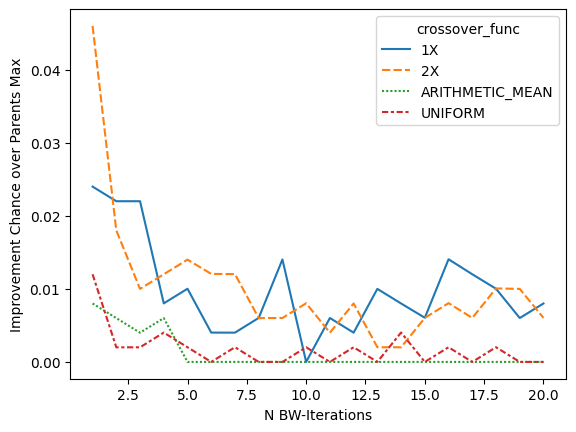
\includegraphics[scale=1.0]{images/charts/crossover_function_improvement_chance_parents_max.png}
%     \end{subfigure}
% \end{figure}



% Zunächst werden wir wir die verschiedenen Vorgeschlagenen genetischen Operatoren miteinander vergleichen bezüglich der Kapazität eine gegebene Lösung zu verbessern. Dazu werden Crossover und Mutationsoperatoren auf Chromosome mit verschiedenen Optimierungsgrad angewendet. Wir können beobachten, dass sowohl Mutation als auch Crossover nur in den seltensten Fällen tatsächlich zu einer Verbesserung führen. Das zeigt, dass wir bei einem genetischen Algorithmus den größten Teil der Rechenleistung darauf verwenden Lösungen zu verschlechtern.

% \section*{Performance Vergleich}
% In diesem Abschnitt vergleichen wir die Performance eines genetischen Algorithmus mit dem Baum-Welch Algorithmus und betrachten welche Schritte des GA-HMM am meißten Rechenzeit beanspruchen. Typischerweise ist bei einem genetischen Algorithmus die Fitnessfunktion am Rechenintensivsten \cite*{MetaheuristicsEGT}. Im Fall des GA-HMM ist die Fitness-Funktion jedoch sehr günstig. Es muss hier angemerkt werden, dass es sich nicht um fairen Vergleich handelt, da die Fitness-Funktion in optimierten C Code implementiert ist und der genetische Teil des GA-HMM nur Teilweise optimiert ist. Ich bezweifle jedoch, dass man die Performance des genetischen Algorithmus stark verbessern kann ohne die Lesbarkeit oder Flexibilität des Codes zu komprimieren. Ein genetischer Algorithmus muss enorm viele Parameter festhalten und wurde daher als Objekt implementiert, welche zumindestens in Python sehr ineffizient sind. Der Baum-Welch Algorithmus hingegen kann als eine einizige Funktion implementiert werden, welche leicht optimiert werden kann. 

% \section*{Implementation verschiedener Ansätze}
% Ja sind alle kacke wer hätte gedacht?

% Richard S. Barr schreibt, dass die Aussagekräftigste Visualiserung eine Darstellung der Qualität gegen Zeit ist.
% Perhaps the most popular and illuminating exhibits of heuristic performance is a graph 
% of solution quality as a function of time.~\cite*{ComparisonGuidelines}
% Daher macht es mich stutzig warum gerade solch eine Visualisierung aus nicht in den Evaluationen der genetischen Algorithmen zu finden ist.


